\label{chapter:improvements}

%%%%%%%%%%%%%%%%%%%%%%%%%%%%%%%%%%%%%%%%%%%%%%
\subsection{Modelling Correlation Functions} %
%%%%%%%%%%%%%%%%%%%%%%%%%%%%%%%%%%%%%%%%%%%%%%

The key insight made by the XPFC model the that, the density-density correlation 
function can be modelled in such a way as to control the crystall lattice structure
targetted under cooling and to target different structures at different concentrations.
Note that the density-density correlation function as the form of a linear combination
of interpolating functions in concentration, $\zeta(c)$, multiplied by bare correlation
functions $C(r, r^\prime)$,
%
\begin{equation}
    C_{nn}(r, r^\prime; c) = \sum_i \zeta_i(c) C_i(r, r^\prime)
\end{equation}
%
In the exact theory, for example, we have,
%
\begin{gather}
    \zeta_{AA}(c) = \rho_0 (1 - c^2), \\
    \zeta_{AB}(c) = \rho_0 c (1 - c ), \\
    \zeta_{BB}(c) = \rho_0 c^2.
\end{gather}
%
Each interpolating function, $\zeta_i(c)$, defines a domain of validity for its
associated correlation function $C_i(r, r^\prime)$. This suggests that we might
model any density-density correlation function using this general structure:
the set of correlation function $C_i(r, r^\prime)$ enumerate the various
structures that may manifest themselves and the associated interpolation
functions $\zeta_i(c)$ define the concentrations over which these correlations
are valid.

As a simple example we wanted to construct a simple model of the silver-cupper
eutectic alloy system, we might start with some model correlation function for
pure silver, $C_\alpha(r, r^\prime)$, and for pure copper, $C_\beta(r,
r^\prime)$. These two structures, the silver rich $\alpha$ phase and the copper
rich $\beta$ phase, are the only two relevent crystalline structures in the
system so to build the full density-density correlation function we just need
to choose interpolating functions for each. Following Greenwood \textit{et al}
for example, we might choose,
%
\begin{gather}
    \zeta_\alpha(c) = 1 - 3c^2 + 2c^3, \\
    \zeta_\beta(c) = 1 - 3 (1 - c)^2 + 2(1 - c)^3.
\end{gather}
%


The regular phase field crystal model is a simplified model that aims to combine 
the positive aspects of the XPFC and original simplified models together. The 
original PFC model uses an regular model of mixing so both enthalpic and entropic 
contribution to the free energy of mixing are considered. This is acheived by
assuming there is a $k=0$ contribution in the gradient expansion of the 
concentration-concentration correlation function. If we add this simple component
to the development of the XPFC free energy functional we find one additional term
that gives an enthaly of mixing,
%
\begin{align}
    \f{\beta\Delta\F[n, c]}{\rho_0} &= \integrate{r} \l\lbrace
        \f{1}{2} n(r) \l(1 - C_{nn}(r, r^\prime)\r) \ast n(r^\prime)
        - \eta \f{n^3}{6} + \chi \f{n^4}{12} \r\rbrace \\
        &+ \integrate{r}\l\lbrace
            \f{1}{2}\l\vert \nabla c(r) \r\vert^2 + \omega f_{mix}(r)
            \r\rbrace. \nonumber
\end{align}
%
Where the local free energy density of mixing, $f_{mix}$ is now,
%
\begin{equation}
    f_{mix}(r) = \l(n(r) + 1\r)\l( 
            c(r)\ln\l(\f{c(r)}{c_0}\r) + (1-c(r))\ln\l(\f{1-c(r)}{1-c_0}\r) \r) + 
            \f{1}{2} \epsilon (c - c_0)^2.
\end{equation}
%
The simplicity the temperature dependence if the parameter $\epsilon$ is taken to be
linear about the spinodal temperature $T_c$,
%
\begin{equation}
    \epsilon(T) = -4 + \epsilon_0(T - T_c).
\end{equation}

%%%%%%%%%%%%%%%%%%%%%%%%%%%%%%%%%%%%%
\subsection{Equilibrium Properties} %
%%%%%%%%%%%%%%%%%%%%%%%%%%%%%%%%%%%%%

Here we'll explore the flexibility of the simplified regular PFC model in
describing various material phase diagrams in binary systems.

%%%%%%%%%%%%%%%%%%%%%%%%%%%%%%%%%%%%%%%%
\subsubsection{Eutectic Phase Diagram} %
%%%%%%%%%%%%%%%%%%%%%%%%%%%%%%%%%%%%%%%%

While previous PFC models have shown that elastic energy is a sufficient
driving force for eutectic solidification our simplified regular model allows
for the examination of the role enthalpy of mixing can play in eutectic solids.
For instance, Murdoch and Schuh noted that in nanocrystalline binary alloys,
while a positive enthaply of segregation can stabilize against grain growth via
solute segregation at the grain boundary, if the enthaply of mixing becomes too
large this effect can be negated by second phase formation or even macroscopic
phase seperation\cite{MURDOCH13}. 

To specialize our simplified regular model to the case of the binary eutectic
we must choose an appropriate model for the correlation function. Choosing an
$\alpha$ phase around $c = 0$ and $\beta$ phase around $c = 1$, we can recover
the pair correlation function used in the binary XPFC with a
particular choice of window functions: 
%
\begin{align}
   \zeta_\alpha(c) &= 2c^3 - 3c^2 + 1 \\
   \zeta_\beta(c) &= \zeta_\alpha(1 - c).
\end{align}
%
Should we choose, for example, an $\alpha$ and $\beta$ phase with 2 dimensional
hexagonal lattices, differing only by lattice constants, we can produce a phase
diagram like that in Fig. \ref{eutectic}.  

\begin{figure}[h]
    \centering	
    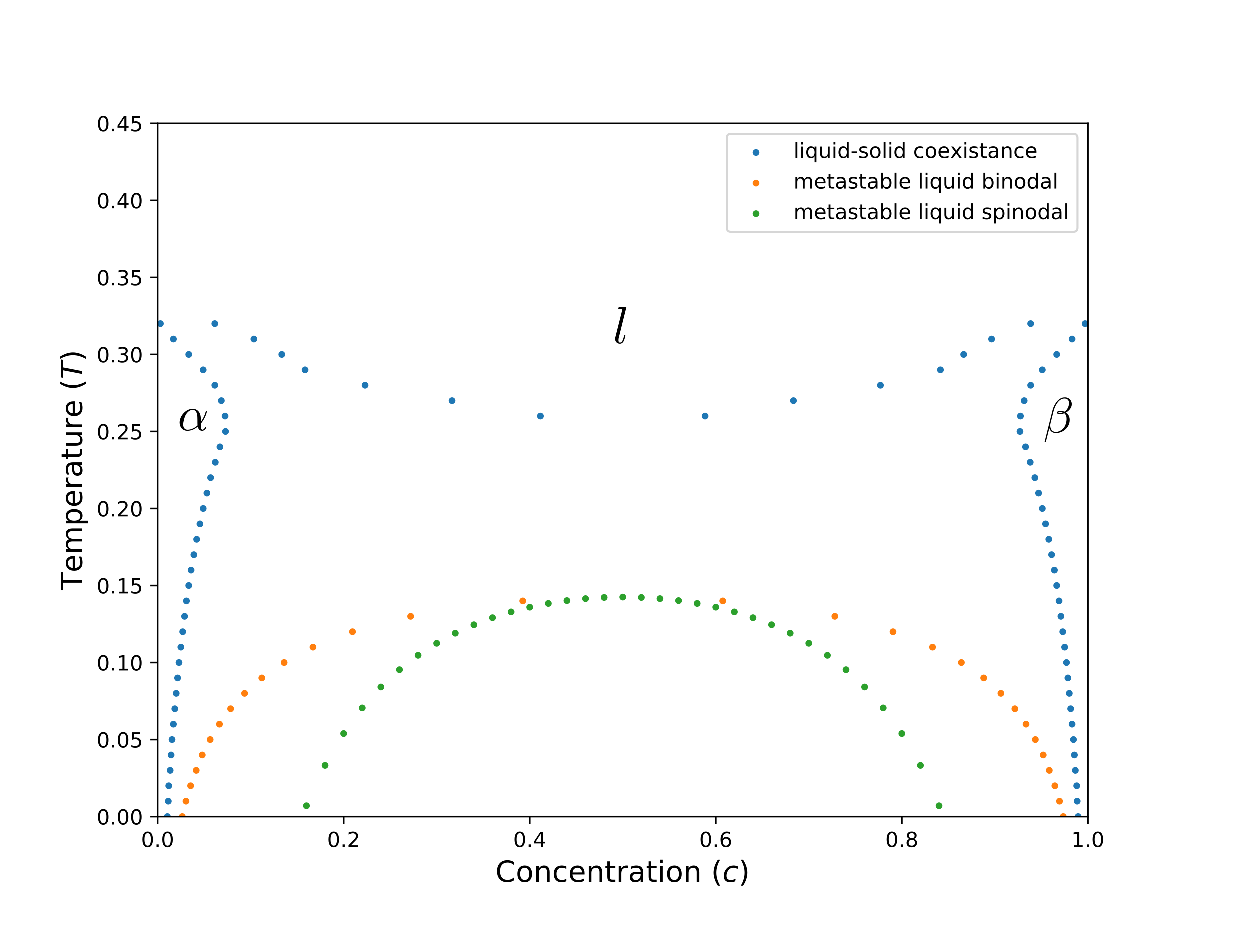
\includegraphics[scale=0.7]{eutectic}
    \caption[Eutectic Phase Diagram]{
        \label{eutectic} Eutectic phase diagram triangle $\alpha$ and $\beta$
        phases. The free energy parameter are $\eta = 2$, $\chi = 1$,
        $\omega=0.30$, $\epsilon_0 = 3$ and $T_c = 0.01$. The parameters of the
        structure functions are $\alpha_{10\alpha} = \alpha_{10\beta} = 0.8$,
        $k_{10\alpha} = 2\pi$, $k_{10\beta} = 4\pi/\sqrt{3}$ and $T_0 = 1$
    }
\end{figure}

%%%%%%%%%%%%%%%%%%%%%%%%%%%%%%%%%%%%%%%%%
\subsubsection{Syntectic Phase Diagram} %
%%%%%%%%%%%%%%%%%%%%%%%%%%%%%%%%%%%%%%%%%

Our regular model also allows for the study of a variety of invariant binary
reactions that, to date, have not been studied using phase field crystal
models. One such reaction is the syntectic reaction. 

The syntectic reaction, $l_1 + l_2 \rightarrow \alpha $, consists of
solidification at the interface of two liquids. We can achieve this with our
model by setting the spinodal temperature, $T_c$, sufficiently high and
producing a density-density correlation function that is peaked at a
concentration below the spinodal. This can be done by choosing a window
function that is centered about an intermediate concentration, $c_\alpha$ of
the solid phase, $\alpha$. 
%
\begin{equation}
  \chi(c) = e^{- \f{(c - c_\alpha)^2}{2 \alpha_c}}
\end{equation}
%
The resulting correlation function for a hexagonal lattice in two dimensions,
for example, would be,
%
\begin{equation}
  \tilde{C}_{nn}(k; c) = 
    e^{-\f{(c - c_\alpha)^2}{2 \alpha_c}}
    e^{-\f{T}{T_0}} 
    e^{-\f{(k - k^\prime)^2}{2\alpha^2}}
\end{equation}
%
A phase diagram that produces a syntectic reaction with an appropriate choice
of parameters can be seen in Fig. \ref{syntectic}.

\begin{figure}
    \centering
	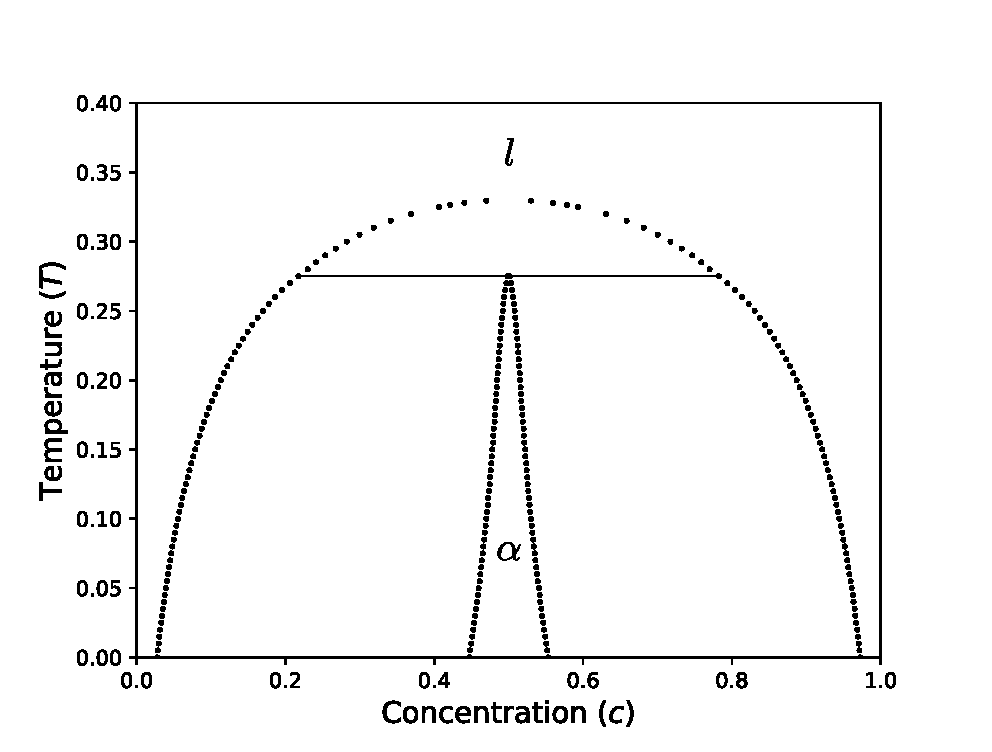
\includegraphics[scale=0.7]{syntectic.eps}
    \caption[Syntectic Phase Diagram]{
        \label{syntectic} Phase Diagram of Syntectic Alloy with a hexagonal
        $\alpha$ phase. The free energy parameters are $\eta=2$, $\chi=1$,
        $\omega=0.3$, $\epsilon_0 = 10$ and $T_c=0.35$. The parameters for the
        structure function are $\alpha_{10\alpha} = 0.8$, $k_{10\alpha} = 2\pi$
        and $T_0 = 1$
    }
\end{figure}

%%%%%%%%%%%%%%%%%%%%%%%%%%%%%%%%%%%%%%%%%%
\subsubsection{Monotectic Phase Diagram} %
%%%%%%%%%%%%%%%%%%%%%%%%%%%%%%%%%%%%%%%%%%

The monotectic reaction is another invariant binary reaction that has not
previously been studied using PFC models. The monotectic reaction, $l_1
\rightarrow \alpha + l_2$, consists of decomposing liquid into a solute poor
solid and solute rich liquid. To model a monotectic using our regular model we
hypothesize a solid phase at $c=0$ and set the spinondal temperature higher
than the solidification temperature. To achieve this we use a window function
peaked around $c = 0$,
%
\begin{equation}
    \chi_\alpha(c) = e^{-\f{c^2}{2\alpha_c^2}}.
\end{equation}
%
Again considering a simple hexagonal lattice for the $\alpha$ phase, we can
produce a phase diagram with a monotectic reaction with an appropriate choice
of parameters as in Fig. \ref{monotectic}.

\begin{figure}
    \centering
	\includegraphics[scale=0.7]{monotectic.eps}
    \caption[Monotectic Phase Diagram]{
        \label{monotectic} Phase Diagram of Monotectic Alloy with hexagonal
        $\alpha$ phase. The free energy parameters are $\eta = 2$, $\chi=1$,
        $\omega=0.3$, $\epsilon_0 = 10$, $T_c = 0.35$ and $c_0 = 0.75$. The
        parameters for the structure function are $\alpha_{10\alpha} = 0.8$,
        $k_{10\alpha} = 2\pi$ and $T_0 = 1$ and the parameter for the window
        function is $\alpha_c = 0.4$
    }
\end{figure}

%%%%%%%%%%%%%%%%%%%%%%%%%%%%%%%%%%%%%%%%%%%%%
\subsubsection{Precipitation from Solution} %
%%%%%%%%%%%%%%%%%%%%%%%%%%%%%%%%%%%%%%%%%%%%%

We can also model precipitation of nanoparticles from solution. While on its
surface the equilibrium phase diagram of a solution is that of a simple
solid-liquid coexistance, in practice the metastable features of the phase
diagram can have profound implications on the nucleation kinetics of
precipitate. As an example, precipitation from solution is a typical synthesis
technique for gold and silver nanoparticles. Recent work by Loh \textit{et al}
shows that a metastable spinodal may be playing an important role in the growth
and nucleation of gold nanoparticles under certain diffusive circumstances.

Using the regular XPFC model we can reproduce the condition of a metastable
liquid spinodal underneath the liquid-solid coexistance curve. The approach to
produce a phase diagram is the same as that of of a monotectic, with the
exception that the spinodal temperature, $T_c$, most now be sufficiently low to
be buried underneath the coexistance curve. In keeping with the concentration
being that of the solute, we'll also center the gaussian window function about
$c = 1$. An example, including metastable spinodal, can be seen in Fig.
\ref{precip}.

\begin{figure}
    \centering	
    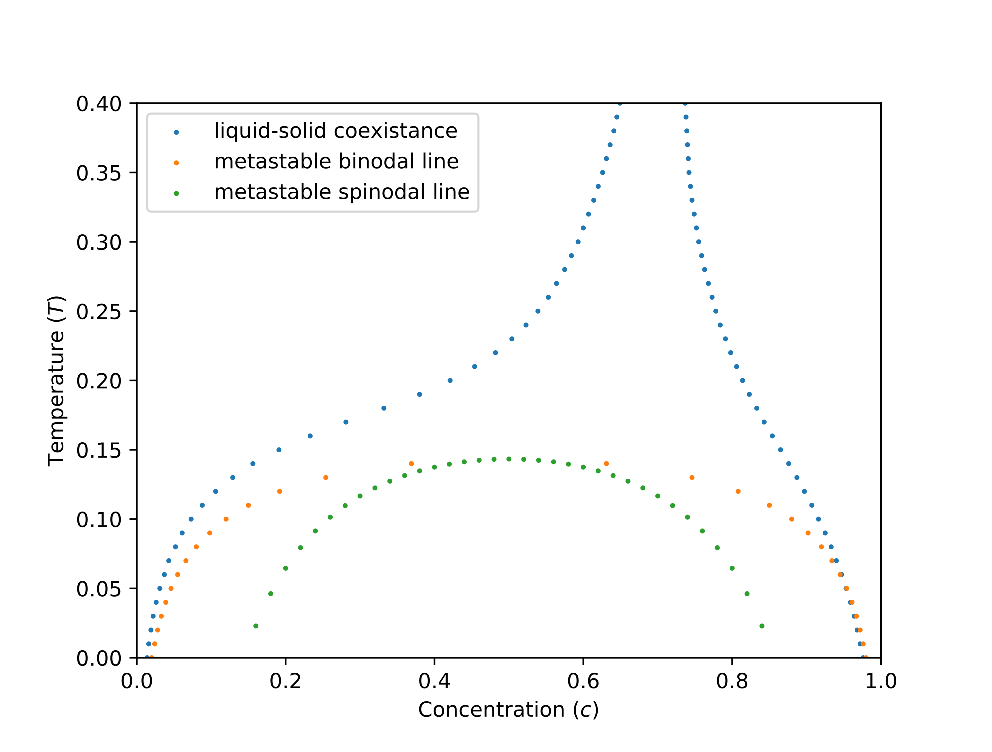
\includegraphics[scale=0.6]{solution.eps}
    \caption[Coexistance Phase Diagram with Metastable Spinodal]{
        \label{precip} Phase Diagram of Solution \color{ForestGreen} fill
        me in please!!
    }
\end{figure}


{
    \color{ForestGreen} Conclude the chapter with discussion of where what we've
    seen and lead into the discussion for the next chapter of dynamics and
    applications of this theory to more than just simple equilibrium 
    phase diagrams
}
